\chapter{Cơ sở lý thuyết} \label{chap:theory}
    \section{Bluetooth Mesh}
    	\subsection{Bluetooth trước Bluetooth Mesh}
Trước khi Bluetooth Mesh ra đời, Bluetooth đã phát triển đến phiên bản 5.0, trong đó có thể chia làm hai giai đoạn (hay hai sứ mạng) bao gồm Bluetooth Basic Rate/Enhanced Data Rate (BR/EDR) và Bluetooth Low Energy (LE). BR/EDR mang lại thế hệ thiết bị không dây mới như tai nghe, chuột, bàn phím không dây,... trong khi đó BLE mang lại các thiết bị chạy pin như đồng hồ thông mình, các thiết bị thể thao, định vị,... Cả hai có thể tồn tại trong cùng một thiết bị nhưng không giao tiếp với nhau.\\

Trong khi BR/EDR chỉ hỗ trợ kết nối 1:1, dễ dàng nhận thấy điều này qua việc một bàn phím không dây không thể dùng cho hai máy tính cùng lúc, hoặc một điện thoại không thể "bắn bluetooth" cho nhiều điện thoại cùng lúc; thì BLE hỗ trợ thêm kết nối 1:nhiều bằng cách thức broadcast, chúng ta có thể tìm thấy kết nối này trong các ứng dụng Bluetooth beacons.
\newpage
       \begin{figure}[h!]
	        	\begin{center}
	        		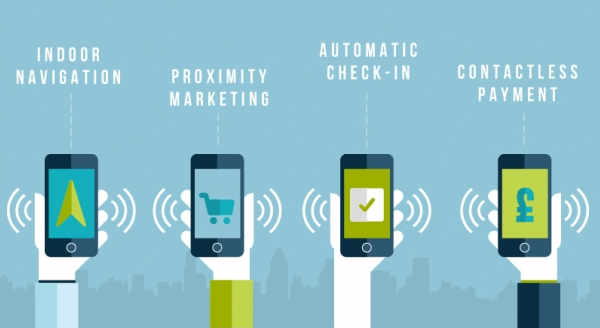
\includegraphics[scale=0.8]{images/retail.png}
	        		\caption{Các ứng dụng sử dụng Bluetooth beacons}
	        	\end{center}
        \end{figure}
        
\textbf{\textit{Vậy Bluetooth Mesh có thể mang lại những tiềm năng gì?}}
    	\subsection{Bluetooth Mesh ra đời}
Bluetooth Mesh được tổ chức SIG đưa ra các giao thức (protocol) chung vào tháng 7 năm 2017\cite{meshborn} và chia sẻ nhiều đặc điểm chung với BLE. Về cơ bản, Bluetooth Mesh sử dụng cấu trúc mạng của BLE nên các thiết bị sử dụng mạng BLE có thể tham gia mạng mesh, cấu hình của các gói tin (package) và phương thức quảng bá (advertisement) của cả 2 giống nhau. Tuy nhiên vẫn có những điểm khác nhau giữa lớp Host của cả 2 mạng. Do đó, Bluetooth là một giao thức kết nối, còn Bluetooth Mesh là một giao thức mạng.
        \begin{figure}[h!]
        	\begin{center}
        		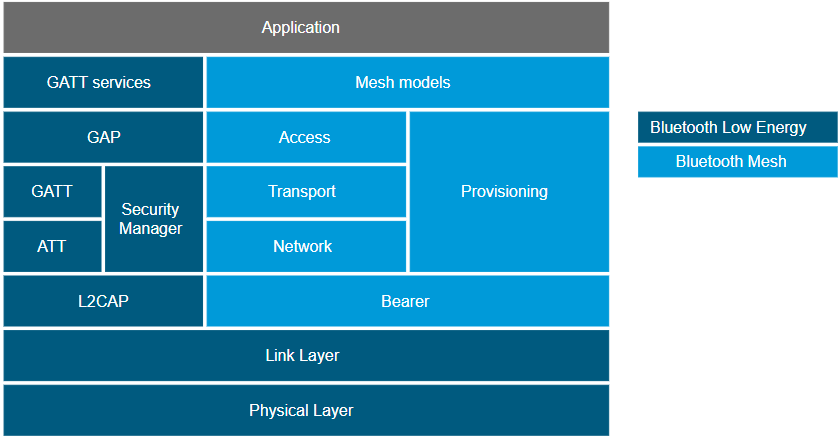
\includegraphics[width=11cm]{images/Bluetooth-mesh-vs-BLE.png}
        		\caption{Mối quan hệ giữa Bluetooth mesh và BLE}
        	\end{center}
        \end{figure}
        \subsection{Sứ mạng của Bluetooth Mesh}
        Bluetooth Mesh hướng đến những ứng dụng điều khiển hoặc giám sát cần các kết nối nhiều:nhiều (một mạng mesh có khả năng phân tán tốt), số thiết bị có thể lên đến hàng ngàn, theo Nordic thì Bluetooth Mesh hỗ trợ tối đa 32767 thiết bị trong một mạng (con số này dựa trên trường địa chỉ mà giao thức BLE Mesh hỗ trợ) với đường kính mạng tối đa là 127 hops\cite{meshconcept}. Chính Nordic đã thử nghiệm trên hệ thống hơn 1000 thiết bị và đạt kết quả khả quan.\\
        
        Định dạng gói tin được tối ưu hóa cho các gói tin nhỏ (kiểu short-burst) chẳng hạn như tắt mở thiết bị, giá trị của số vài cảm biến, giá trị độ sáng bóng đèn,... không dành cho việc truyền dữ liệu hoặc các ứng dụng băng thông cao khác như streaming nhạc và video.
        \begin{figure}[h!]
        	\begin{center}
        		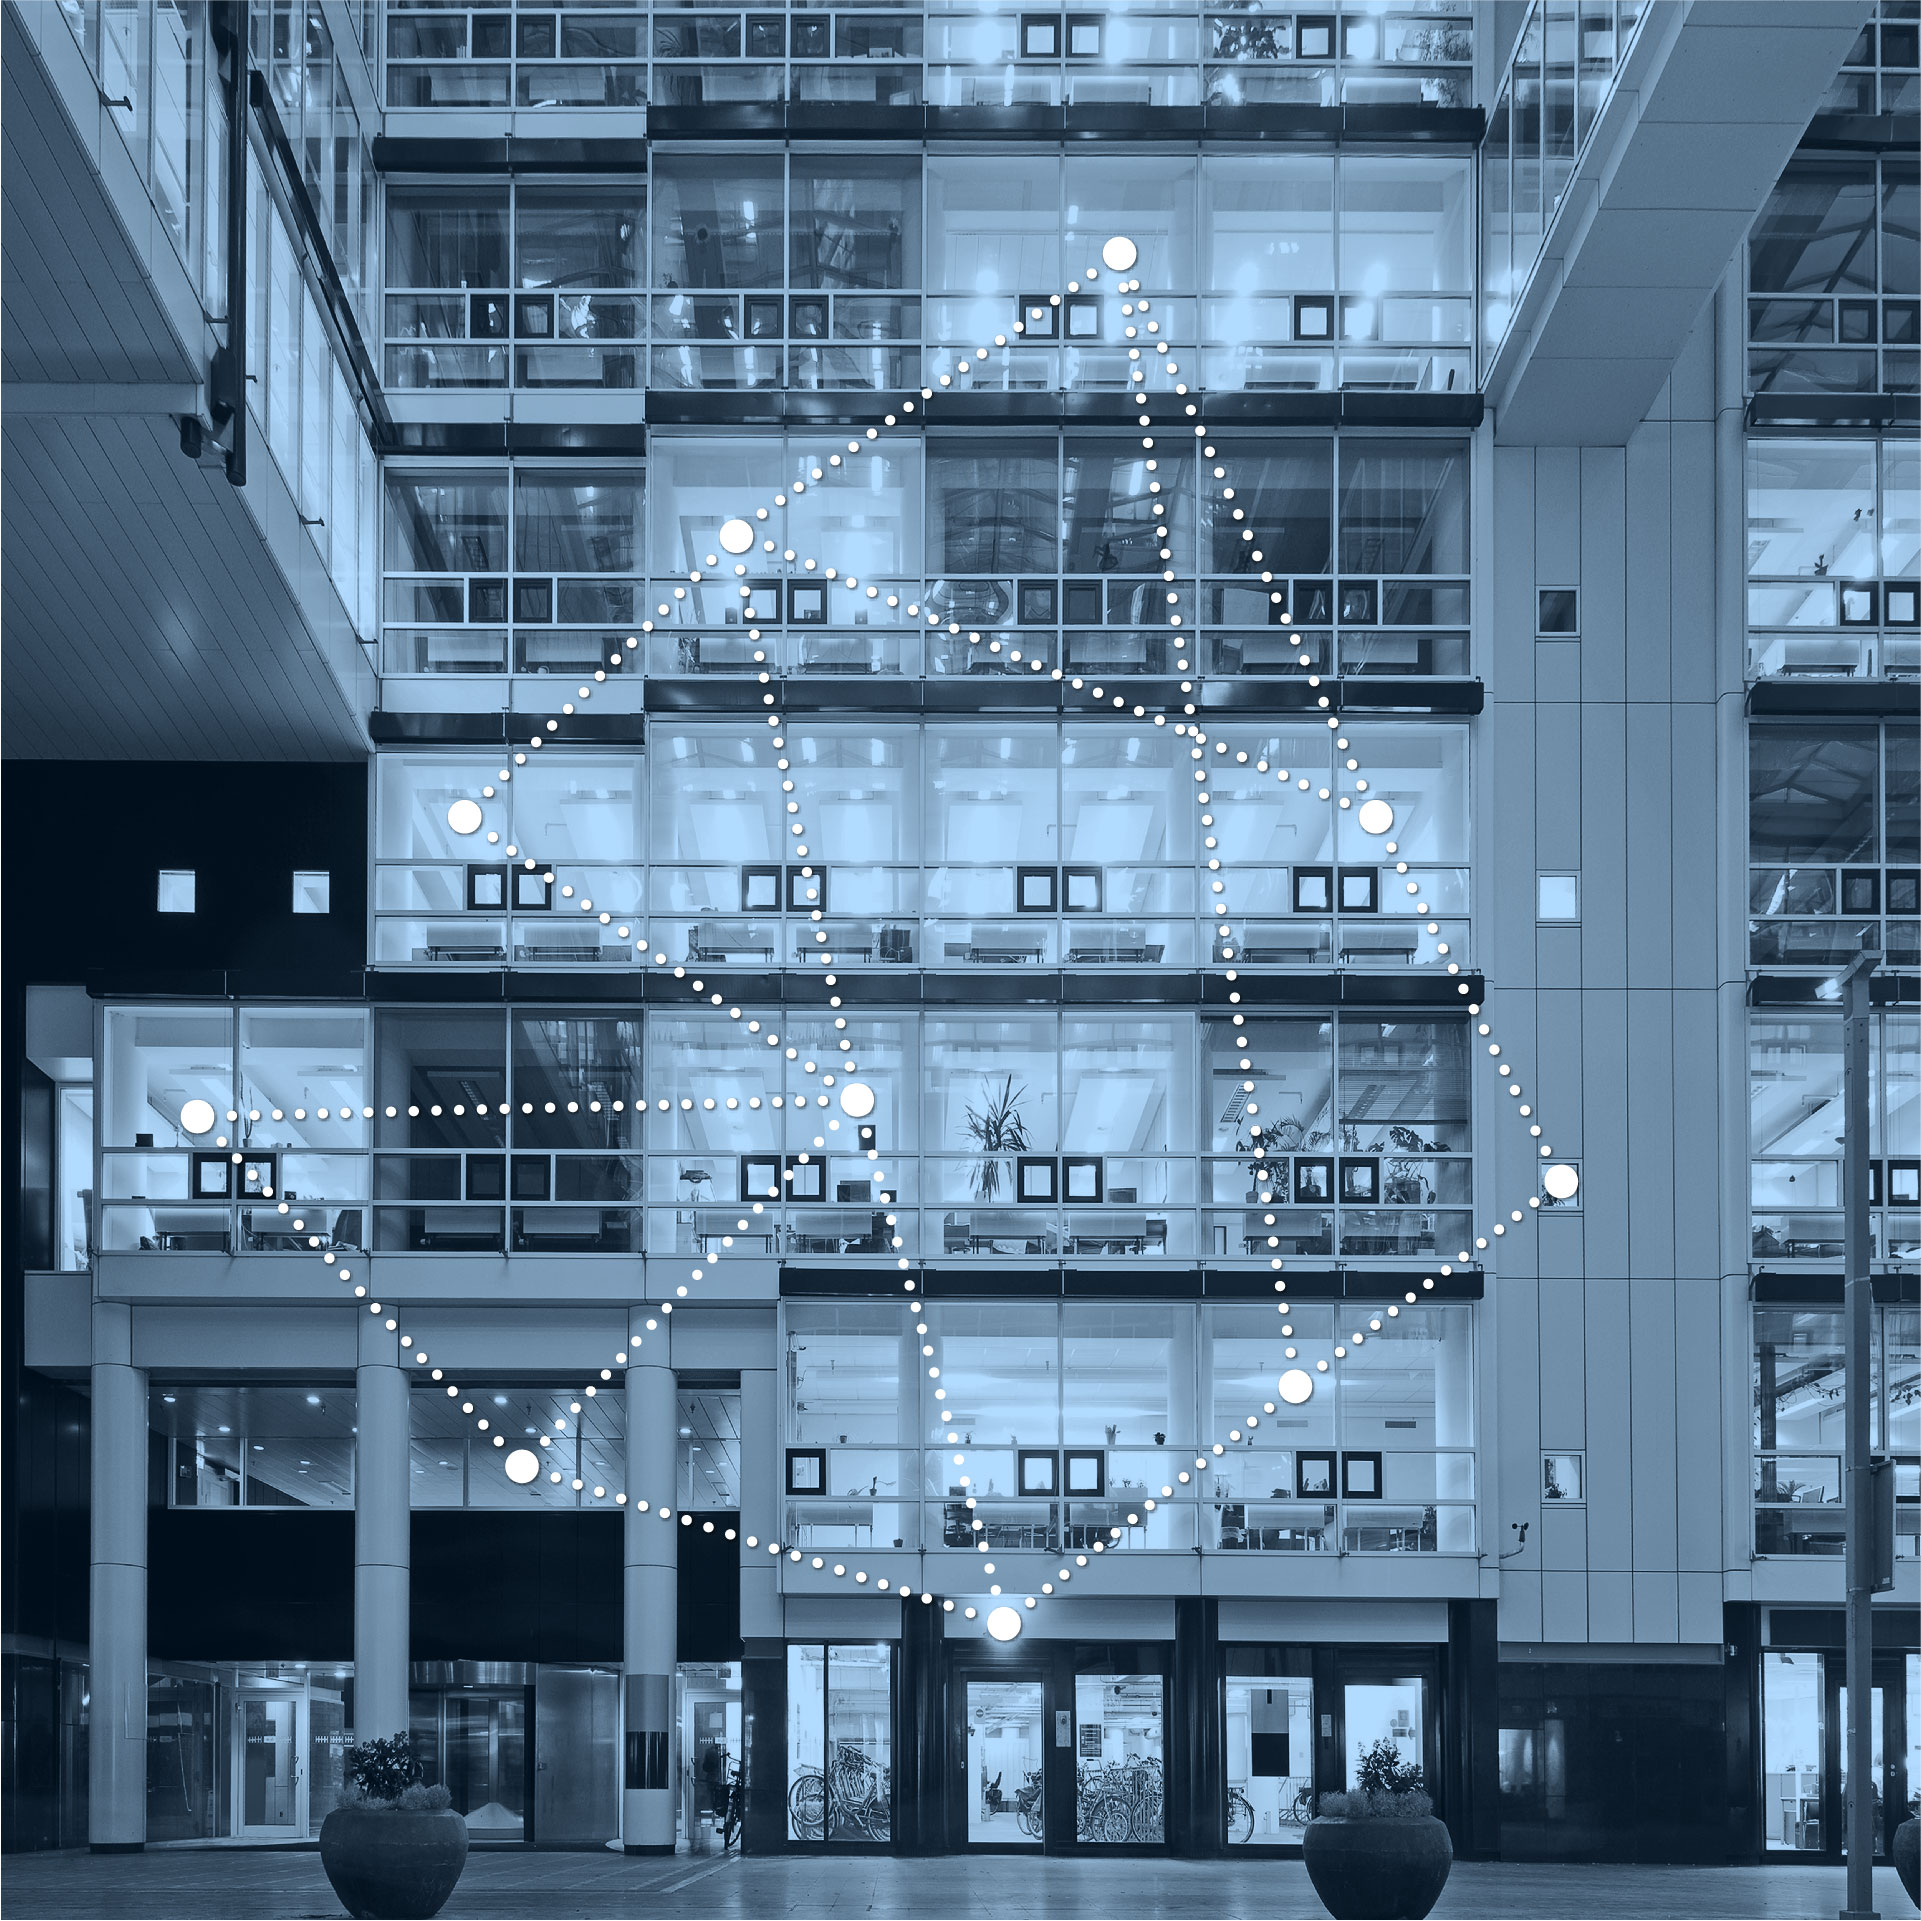
\includegraphics[scale=0.2]{images/Office_4_square_LE-mesh.jpg}
        		\caption{Hệ thống đèn của một tòa nhà ứng dụng Bluetooth Mesh}
        	\end{center}
        \end{figure}
        
    \section{Ưu điểm của Bluetooth Mesh}
    Để tiến hành triển khai các ứng dụng IoT trong thực tế, vấn đề bảo mật là cực kỳ quan trọng, đặc biệt trong các ngành y tế, giao thông và an ninh, hiện nay các hệ thống IoT sử dụng các giao thức thông thường như WiFi, Ethernet, GSM bị xem là bảo mật kém. Kể cả trong các ứng dụng điều khiển trong nhà thì việc một người lạ có quyền tắt mở đèn, quạt trong nhà của chúng ta thì cũng đủ mang lại nhiều phiền phức rồi. \\
    
    Vấn đề liên kết giữa các nhà sản xuất cũng quan trọng không kém, chẳng hạn chúng ta mua một bộ gồm đèn và remote của hãng A, sau một thời gian thì thấy đèn của hãng ko bền nên muốn dùng đèn của hãng khác, nhưng remote của hãng A lại không điều khiển được đèn của hãng khác mà mua một remote khác thì tốn kém hơn mua đèn nhiều.\\
    
    Ngoài ra còn hai vấn đề không kém phần quan trọng là tính mở rộng và khả năng tiết kiệm năng lượng, tuy nhiên hai vấn đề này lại phụ thuộc vào các ứng dụng thực tế, một số ứng dụng thì cần nhưng một số lại không. Chẳng hạn như những hệ thống nhỏ, có số lượng thiết bị không đáng kể thì không cần thiết có khả năng mở rộng; những ứng dụng như hệ thống đèn có khả năng kết nối trực tiếp với mạng điện lưới thì tiết kiệm năng lượng trở nên không mấy quan trọng.\\
    
     \textbf{Bluetooth Mesh là giải pháp hội đủ cả bốn tiêu chí trên, rất thích hợp để làm nền tảng triển khai các ứng dụng từ công nghiệp cho đến dân dụng.}
        \subsection{Tính bảo mật}
            \begin{itemize}
                \item Bluetooth Mesh dùng 3 key để mã hóa: Devive Key, Application Key và Network Key dùng để mã hóa gói tin ở lớp network và application. NetKey giúp chia một mạng mesh thành nhiều subnet, chẳng hạn như subnet trong nhà và subnet ngoài vườn, do tính năng relay gói tin được hiện thức ở lớp Network nên nếu không cùng NetKey thì không thể relay, nghĩa là khác subnet sẽ không truyền tin qua lại được. Như vậy một mạng mesh có thể dùng nhiều NetKey trong đó có một NetKey cho toàn mạng và nhiều NetKey cho các subnet. AppKey mã hóa ở 2 lớp trên cùng là Model và Foundation Model, do đó chỉ có người nhận mới đọc được gói tin ở lớp này.
                \item NetKey còn được dùng để tạo ra Privacy Key, key này dùng để xáo trộn header của gói tin khiến cho kẻ tấn công không thể xác định địa chỉ nguồn, địa chỉ nhận.
                \item Mỗi gói tin đều có trường authentication (một cách chứng minh gói tin này xuất phát từ một node trong mạng) dài 64-bits, có thể tăng thêm.
                \item Chống tấn công kiểu relay bằng cách bắt buộc chỉ số sequence phải thay đổi mỗi lần gửi tin, ngoài ra còn hỗ trợ thêm một trường nonce như một cách redundant, trường này sẽ được tạo mới mỗi khi gửi nhận tin dựa trên 2 thông số là Initialisation Vector (IV) index và chỉ số sequence. Mỗi khi bộ đếm sequence gần cạn kiệt (tràn số hoặc không thể tạo ra nonce mới, nonce mới ở đây yêu cầu phải khác tất cả nonce cũ), lúc này sẽ tiến hành quy trình cập nhật IV cũng tương tự quy trình tạo mới key chống trashcan dưới đây.
                \item Chống tấn công kiểu brute-force bằng độ dài key vào mạng 128-bits, trường authentication 64-bits.
                \item Chống tấn công kiểu man-in-the-middle (MITM) bằng cách áp dụng quy trình trao đổi key ECDH\cite{ECDH} cùng với out-of-band authentication (xác thực thông qua một bên thứ ba, có thể là một kênh giao tiếp khác).
                \item Chống tấn công kiểu trashcan: kẻ tấn công lấy thông tin như key vào mạng từ một node bị hỏng hoặc lỗi nên bị loại khỏi mạng. Cách thức chống kiểu tấn công này sẽ được thảo luận trong phần \ref{removenode}.
                \item Chống tấn công kiểu vật lý: vì Bluetooth Mesh hỗ trợ mạng lưới thiết bị rộng lớn nên không tránh khỏi việc một số node không an toàn về vật lý: đèn ở ngoài vườn có độ an toàn vật lý thấp hơn hẳn đèn trong phòng ngủ, do đó kẻ tấn công có thể khai thác lỗ hổng này bằng cách tấn công vào node kém an toàn và từ đó điều khiển toàn bộ mạng. Bluetooth Mesh có khả năng phân loại key: key dành cho nhóm kém an toàn khác với key của nhóm an toàn nên các node kém an toàn không điều khiển được các node an toàn.
                \item Chống tấn công kiểu visitor bằng cách cấp cho các node tạm (trong một số ứng dụng sẽ phát sinh các node cần truy cập tạm thời vào mạng để gửi nhận thông tin) key có thời gian sống giới hạn, sau một thời gian node tạm không còn khả năng truy cập mạng nữa.
                \item Ngoài ra các gói tin còn được xác thực bằng các thuật toán như AES-CMAC, AES-CCM,...
            \end{itemize}
        \subsection{Tính liên kết}
        Bluetooth Mesh có khả năng liên kết các nhà cung cấp với nhau. WiFi và Zigbee đang được sử dụng phổ biến trong các giải pháp mà Bluetooth Mesh dự định thay thế: smart building, smart home,... nhưng lại thiếu sự tương tác giữa các nhà cung cấp. Các thiết bị của hai hãng khác nhau không thể giao tiếp với nhau, do cấu trúc lệnh của mỗi hãng là do họ tự định nghĩa. Đối với Bluetooth Mesh thì khác, SIG đã định nghĩa sẵn các model như cách BLE đã làm với các profile chuẩn, các nhà sản xuất chỉ việc làm theo đúng chuẩn đó thì điều khiển hãng này dùng cho bóng đèn hãng khác không còn là vấn đề.
        \subsection{Dễ mở rộng}
        Do đặc thù là mạng mesh nên ưu điểm của Blueetooth Mesh sẽ là tính phân tán, các node không cần phải đặt tập trung vào một gateway hay access point mà có thể đặt bất cứ nơi đâu tùy theo nhu cầu ứng dụng. Khi áp dụng giao thức BLE Mesh vào trong IoT, phạm vi hoạt động của mạng lưới cảm biến sẽ được mở rộng rất nhiều, chẳng hạn như node A nằm ngoài phạm vi kết nối của node B, tuy nhiên chỉ cần đặt thêm node C vào giữa hai node này, thế là A có thể giao tiếp với B thông qua C, thử tưởng tượng với 127 hops mà khoảng cách giữa 2 node khoảng 8 - 10m (kết quả thử nghiệm thực tế), phạm vi tối đa sẽ đạt tới mức nào? 
        \subsection{Tiết kiệm năng lượng}
        Bluetooth Mesh là giao thức mạng, kết thừa các lớp của BLE nên cũng kế thừa khả năng tiết kiếm năng lượng. Ngoài ra, Bluetooth Mesh còn đưa ra khái niệm Friendship, giúp cho các node cần tiết kiệm năng lượng  có thể ở trạng thái sleep lâu hơn mà không bị loại ra khỏi mạng hoặc bỏ lỡ những gói tin được gửi tới nó. 
        \subsection{Một số ưu điểm khác của Bluetooth Mesh}
        \begin{itemize}
            \item Bluetooth Mesh đạt các yêu cầu cho một ứng dụng công nghiệp với đầy đủ các yêu cầu: đáng tin cậy (reliability), dễ mở rộng (scalability) và tính bảo mật cao.
            \item Sản phẩm dễ được thị trường đón nhận hơn vì Bluetooth đã trở thành thường thức với phần đông dân số thế giới, do đó khi nhà sản xuất miêu tả sản phẩm này áp dụng giao tiếp Bluetooth thì khách hàng dễ hình dung hơn là Zigbee hay Lora nhiều.
            \item Chức năng Bluetooth vốn tích hợp sẵn trên mọi chiếc điện thoại thông minh, thậm chí điện thoại không thông minh, cũng như rất nhiều thiết bị công nghệ như máy tính bảng, laptop,... Mức độ phổ biến của nó tương ứng với tiềm năng phát triển trong tương lai, khi mà Bluetooth Mesh chấp nhận giao tiếp với thiết bị non-mesh (các thiết bị dùng Bluetooth hiện nay đều là non-mesh), mà theo như thông tin nhóm tìm hiểu thì các một số thiết bị BLE từ 4.0 trở lên và có đủ điều kiện (chẳng hạn như dung lượng bộ nhớ còn trống trong chip) thì có thể giao tiếp với một mạng mesh thông qua ứng dụng.
            \item Khi mạng lưới càng lớn thì khả năng tự hồi phục của mạng càng mạnh, việc một vài node bị hỏng sẽ không ảnh hưởng tới mạng bất kể node đó có phải relay hay không, bởi vì còn rất nhiều con đường khác - những node relay khác - để gói tin có thể đi qua.
            \item Khả năng thiết lập kết nối nhanh, khi có phần tử mới muốn tham gia vào mạng, chỉ cần được thiết lập với key hợp lệ.
            \begin{figure}[h!]
        	    \begin{center}
        		    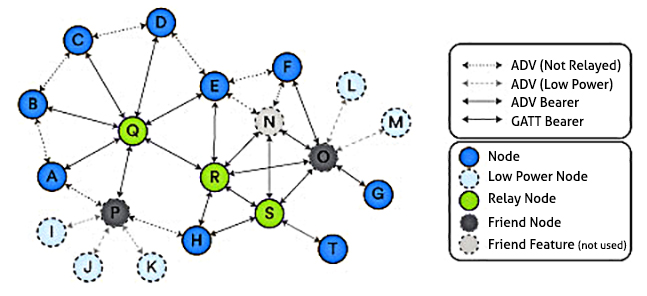
\includegraphics[scale=1.0]{images/mesh-topo.jpg}
        		    \caption{Mạng mesh với node "bạn bè" và low power}
        	    \end{center}
            \end{figure}
        \end{itemize}
        \newpage
    \section{Kiến trúc Bluetooth Mesh}
    Trong phần này, nhóm sẽ trình bày những đặc điểm chính của từng thành phần trong kiến trúc Bluetooth Mesh. Mô hình kiến trúc được thể hiện trong hình bên dưới:
    
    \begin{figure}[h!]
    	\begin{center}
    		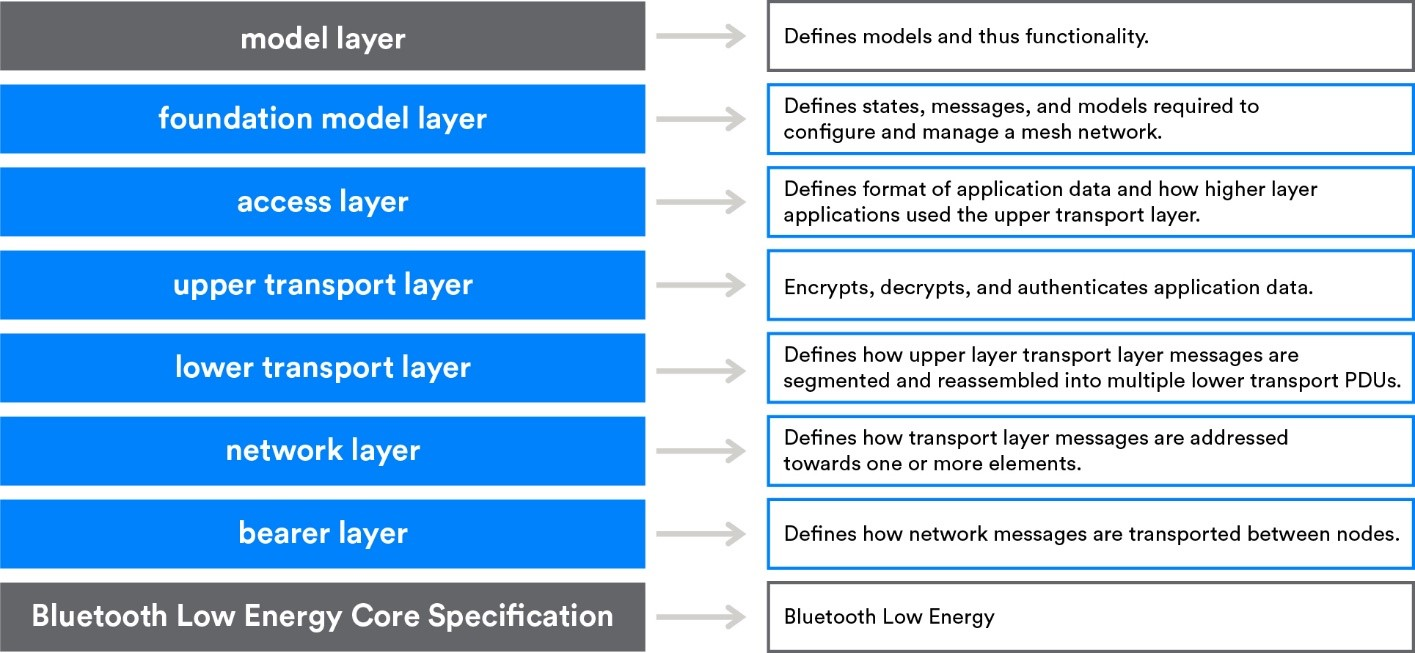
\includegraphics[scale=0.8]{images/mesh-architexture.jpg}
    		\caption{Kiến trúc Bluetooth mesh}
    	\end{center}
    \end{figure}
    
    \subsection{Lớp Model}
    Lớp model chịu trách nhiệm hiện thực các model, nghĩa là hiện thực các hành vi, trạng thái, gói tin điều khiển,... Tham khảo thêm về các model chuẩn trong phần phụ lục \ref{models}.
    \subsection{Lớp Foundation Model}
    Lớp Foundation Model như một lớp đệm cho lớp Model, thiết lập và quản lý lớp Model cho thích hợp với mạng mesh.
    \subsection{Lớp Access}
    Lớp Access kết nối và giúp 2 lớp trên (lớp Model và Foundation Model, nếu gộp 2 lớp này lại thì giống với lớp Apllication trong mô hình OSI) sử dụng tài nguyên là các lớp bên dưới.
    \begin{itemize}
        \item Định nghĩa cấu trúc của 2 lớp trên
        \item Định nghĩa và điều khiển quá trình mã hóa, giải mã trong lớp Upper transport
        \item Kiểm tra và xác nhận gói tin được gửi từ lớp Upper transport là đúng mạng và đúng ứng dụng trước khi chuyển lên lớp cao hơn
    \end{itemize}
    \subsection{Lớp Upper Transport}
    Lớp Upper transport chịu trách nhiệm mã hóa, giải mã và xác thực gói tin chuyển xuống (lúc gửi) hoặc trước khi chuyển lên (lúc nhận) lớp Access. Lớp này cũng chịu trách nhiệm tạo ra và vận chuyển các gói tin đặc biệt qua lại giữa các node: bao gồm các gói tin liên quan đến friendship và heartbeats.
    \subsection{Lớp Lower Transport}
    Lớp Lower transport nhận gói tin từ lớp Upper transport layer và chia nhỏ nếu gói tin quá dài, vượt quá giới hạn của lớp này. Trong trường hợp nhận, lớp Lower transport sẽ chịu trách nhiệm ghép gói tin lại nếu nó đã bị chia nhỏ, sau đó chuyển lên lớp trên.
    \subsection{Lớp Network}
    Lớp Network định nghĩa các kiểu địa chỉ (unicast, vitural, group) cũng như cấu trúc của gói tin ở lớp này, cho phép gói tin từ lớp Transport đi xuống lớp Bearer. Lớp này hỗ trợ nhiều bearer (một dạng kênh truyền), trong đó mỗi bearer lại mang nhiều network interface, network interface là cách để các element của các node giao tiếp với nhau, bao gồm cả các element trong cùng 1 node (local network interface). \\
    
    Lúc gửi dữ kiệu lớp Network layer sẽ quyết định gửi gói tin tới network interface nào, sau đó lớp này sẽ thông qua bộ lọc để lọc các dữ liệu được đưa xuống lớp Bearer. Lúc nhận gói tin từ lớp Bearer, một bộ lọc sẽ lọc xem gói tin nào sẽ được đưa tiếp lên lớp trên (khi đúng network interface), gói tin nào sẽ bỏ qua. Tính năng Relay và Proxy được hiện thực ở lớp Network.
    \subsection{Lớp Bearer}
    Các gói tin mesh cần một nền tảng để gửi nhận, nền tảng đó chính là BLE, lớp Bearer sẽ định nghĩa cách các gói tin được xử lý và vận chuyển. Hiện nay có hai Bearer là Advertising Bearer và GATT Bearer.\\
    
    Advertising Bearer kế thừa tính năng quảng bá (advertising) và dò tìm (scanning) của BLE GAP để gửi nhận các gói tin mesh. Còn GATT Bearer cho phép các thiết bị không hỗ trợ Advertising Bearer giao tiếp gián tiếp với các node trong mạng mesh thông qua giao thức Proxy. Node sử dụng giao thức này gọi là node Proxy, node sử dụng Proxy và node sử dụng Advertising Bearer có thể giao tiếp với nhau một cách bình thường.\\
    
    Giao thức Proxy sử dụng profile GATT vốn là profile cơ bản nhất của BLE, trong đó giao thức này sẽ sử dụng một số characteristics được định nghĩa sẵn để giao tiếp (Mesh Proxy Data). Gói tin sẽ được write vào characteristics Mesh Proxy Data In của node proxy, gói tin sẽ được lấy ra từ characteristics Mesh Proxy Out.
     \section{Nguyên lý hoạt động của Bluetooth Mesh}
            \subsection{Phần tử trong mạng}
            Mỗi thiết bị tham gia trong mạng được gọi là một node, trong một ứng dụng thực tế thì mỗi một node đều có thể có nhiệm giống hoặc khác nhau, chẳng hạn như node đọc giá trị cảm biến do tính chất đọc theo chu kỳ nên có thể dùng nguồn pin và chạy low power, node gateway lại cần cấp nguồn liên tục để cập nhật tình hình với server,... Trong mạng Bluetooth Mesh có 4 loại node đặc biệt như sau:
            \begin{itemize}
                \item Low-power: tiêu tốn năng lượng cực thấp, có thể hoạt động trong vòng vài năm với nguồn pin coin (coin battery).
                \item Friend: bắt buộc phải có nếu trong mạng có node low-power, bởi vì mỗi khi node low-power muốn giao tiếp, nó sẽ chỉ giao tiếp với node friend của nó, còn node friend có nghĩa vụ lưu lại những dữ liệu mà các node khác gửi cho node low-power. Do đó node friend cần cấp nguồn liên tục.
                \item Relay: node relay sẽ broadcast bất cứ dữ liệu nào được gửi đến nó mà nó ko phải người nhận duy nhất, giúp mở rộng mạng mesh. Node relay cũng cần cấp nguồn liên tục.
                \item Proxy: node này liên kết các node trong mạng mesh với các thiết bị sử dụng BLE và không nằm trong mạng mesh, node proxy cũng cần năng lượng và thêm khả năng tính toán của vi xử lý.
            \end{itemize}
            \newpage
            Dù các node có hay không 4 chức năng trên, cấu trúc một node cũng gồm nhiều thành phần nhỏ hơn được thể hiện trong các hình sau:
            \begin{figure}[h!]
            	\begin{center}
            		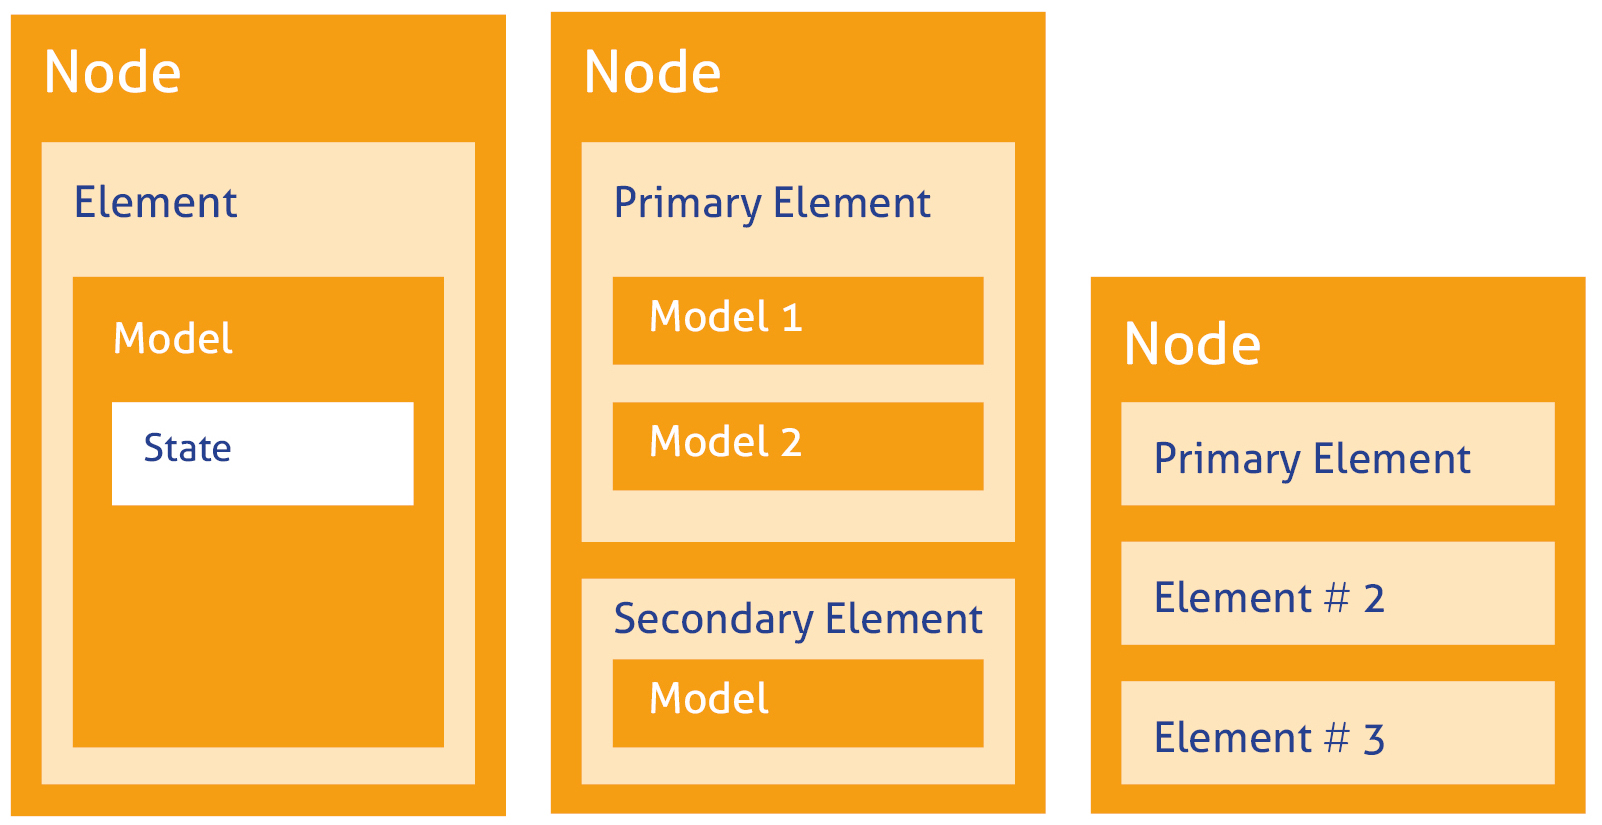
\includegraphics[scale=0.2]{images/mesh-node.jpg}
            		\caption{Cấu trúc của một node}
            	\end{center}
            \end{figure}

            Mỗi node phải gồm ít nhất một element - element sẽ định nghĩa các state (trạng thái) hoặc chức năng (functionality) của node. Ví dụ một node điều khiển nhiều thiết bị, các thiết bị là các element và mỗi element lại có nhiều trạng thái khác nhau, mỗi trạng thái là một model (model server). Hình bên dưới minh họa element đèn bao gồm 2 model trạng thái đèn và model độ sáng đèn.
            \begin{figure}[h!]
            	\begin{center}
            		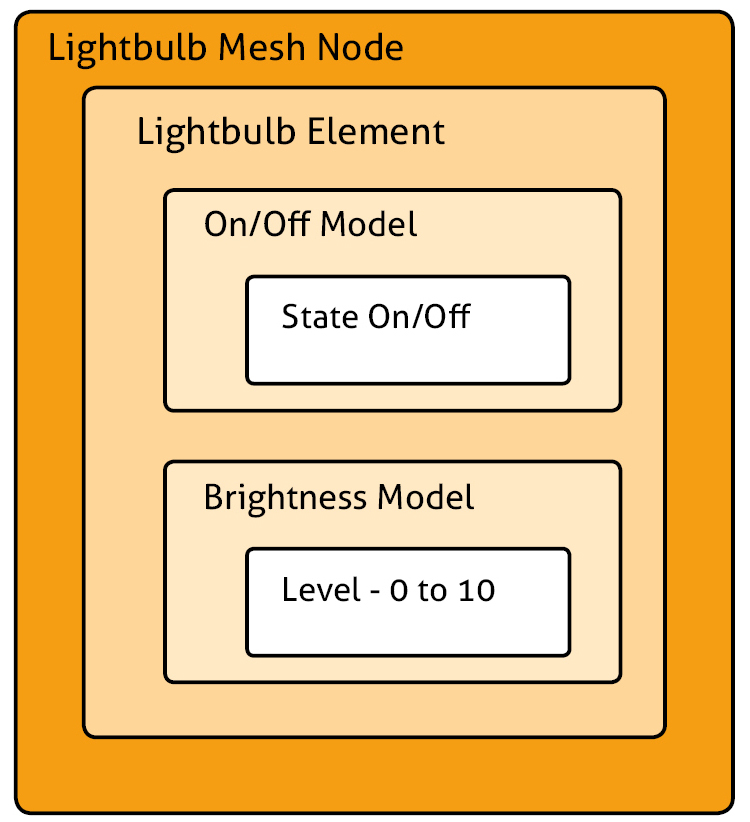
\includegraphics[scale=0.2]{images/lighbulb-node.jpg}
            		\caption{Cấu trúc của một node bóng đèn}
            	\end{center}
            \end{figure}

            Các model trong giao thức Bluetooth Mesh được phân làm 3 loại:
            \begin{itemize}
                \item Server: thể hiện trạng thái, như trong ví dụ trên. Sau đó nhận tin từ các node khác để thay đổi trạng thái và xuất tín hiệu ra các chân I/O, PWM tương ứng.
                \item Client: thể hiện chức năng, bao gồm các hàm có chức năng thay đổi trạng thái của các model server.
                \item Control: thể hiện cả trạng thái và chức năng, cộng thêm liên hệ logic giữa trạng thái và chức năng. Ví dụ một model control quạt dựa vào nhiệt độ, model này có chức năng lấy dữ liệu nhiệt độ từ cảm biến (của một node khác), sau đó kiểm tra ngưỡng rồi quyết định bật hay tắt quạt.
            \end{itemize}

            Trong đề tài này node gateway sẽ dùng model Simple OnOff client, node cảm biến sẽ dùng model Simple OnOff server. Node cảm biến lưu giữ trạng thái đèn (nhóm đã cải tiến thành lưu giữ giá trị cảm biến, xem phần \ref{simpleonoff}), node gateway sẽ đọc dữ liệu này để gửi lên server, nhóm có hiện thực thêm chức năng client gửi tín hiệu tắt/mở LED để tiện demo. Do đó có hiện tượng cùng một biến 8-bits nhưng có lúc lưu giữ giá trị cảm biến, có lúc lưu trạng thái đèn.
            \subsection{Truyền tin trong mạng}
            Bluetooth Mesh dùng cơ chế flooding để lan truyền gói tin, nghĩa là gói tin cần gửi sẽ được boardcast ra các node xung quanh, các node được boardcast sẽ kiểm tra mình có phải người nhận hay không, nếu không thì tiếp tục boardcast (còn gọi là relay, các node relay cần cung cấp nguồn đầy đủ và liên tục) cho đến khi tới được người nhận nếu là địa chỉ là unicast (hoặc một nhóm nhận nếu là địa chỉ multicast). Quá trình flooding này dừng lại khi đạt giới hạn 127 hops hoặc vượt quá thông số Time To Live (TTL) - thông số này tương đương số lần gói tin được relay\cite{meshgloss}.\\
            Sau đó, Bluetooth Mesh dùng cơ chế publish-subscribe để các gói tin tới được nơi cần tới. Các địa chỉ unicast được đánh cho các element trong node và được gọi là publish address, còn có multicast address và vitural address bao gồm nhiều element (địa chỉ multicast thường đại diện cho cho một tầng lầu, một phòng,... trong thực tế). Khi có tin mới được gửi đến một địa chỉ publish address, bất kỳ những model nào (element bao gồm nhiều model) trong element và có đăng ký nhận tin (subscribe) ở địa chỉ đó sẽ nhận được tin.
        
            \begin{figure}[h!]
        	    \begin{center}
        		    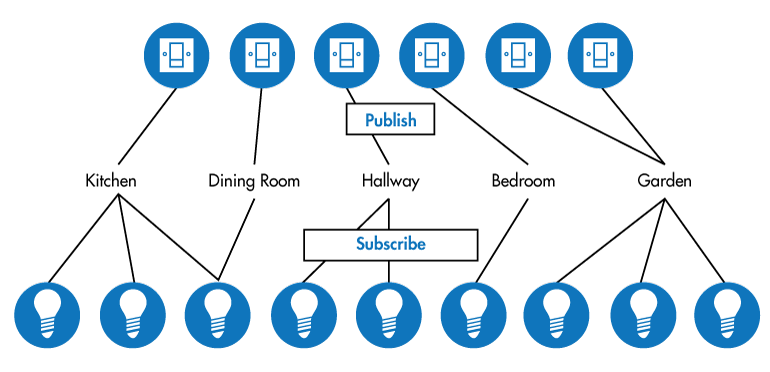
\includegraphics[scale=0.5]{images/mesh-pub-sub.png}
        		    \caption{Sơ đồ của cơ chế publish-subscribe}
        	    \end{center}
            \end{figure}
    \section{Quản lý các phần tử trong mạng}
        \subsection{Tham gia mạng - Provisioning}
            Để một thiết bị mới tham gia vào mạng mesh, cần thực hiện quá trình provisioning. Đây cũng được xem như quá trình bắt tay giữa các thiết bị khi tham gia vào mạng mesh, sau khi hoàn thành quá trình provionsing gồm 5 bước, thiết bị chính thức trở thành node - một thành phần trong mạng. Bluetooth Mesh hỗ trợ hai cách để provision một thiết bị:
            \begin{itemize}
                \item PB-ADV: Sử dụng gói advertising của BLE để tiến hành provisioning bằng cách thay đổi một số trườngww.
                \item PB-GATT: Sử dụng các characteristics của GATT để tiến hành provisioning, chỉ dùng khi thiết bị mới không hỗ trợ advertising hoặc không cho tùy chỉnh gói advertising.
            \end{itemize}

            Ngoài ra, khi thiết bị mới nằm ngoài tầm phủ sóng của provisioner, Bluetooth cũng hỗ trợ provisioning thông qua các node trung gian hoạt động như các relay để gửi các gói tin liên quan provisioning, quá trình này gọi là remote provisioning. Quá trình này có thể không cần thiết trong đa số ứng dụng trong thực tế vì người dùng hoàn toàn có thể mang theo thiết bị provionser như smartphone, sau đó đặt thiết bị mới vừa tầm và tiến hành provisioning. Có thể tham khảo flowchart của quá trình này trong phần \ref{remoteprov}.

            \begin{figure}[h!]
            	\begin{center}
            		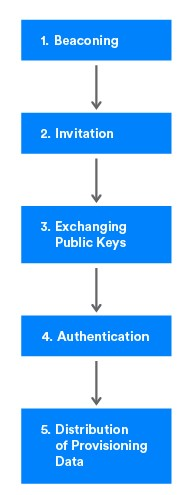
\includegraphics[scale=0.8]{images/mesh-management-fig2.jpg}
            		\caption{Quá trình provisioning gồm 5 bước}
            	\end{center}
            \end{figure}

            Tiếp theo, nhóm sẽ trình bày chi tiết hơn về quá trình provisioning thông qua PB-ADV:
            \begin{itemize}\label{security}
                \item Bước 1 - Beaconing: Khi một thiết bị mới (unprovisioned) muốn gia nhập mạng mesh, thiết bị này sẽ cần Network Key của mạng đó, sau đó tiến hành phát beacon để thông báo sự hiện diện của mình, tùy nhà sản xuất mà quá trình có thể kích hoạt bằng cách nhấn hoặc giữ nút,... Lúc này thiết bị đóng vai trò provisioner - thường sẽ là điện thoại, máy tính bảng có cài ứng dụng đặc biệt - sẽ tiến hành scan thiết bị mới, khi provionser phát hiện được thiết bị mới thì tiến hành bước tiếp theo. Trong đề tài này, nhóm sử dụng node gateway để thực hiện chức năng provisioning vì chưa phát triển được ứng dụng trên điện thoại.
                \item Bước 2 - Invitation: Provisioner sẽ gửi một lời mời, một gói tin Provisioning Invite PDU, đến thiết bị cần provisioning, thiết bị này sẽ đáp lại bằng một gói Provisioning Capabilities PDU, trong đó chứa một số thông tin của nó như số element,... đặc biệt là các input output mà nó hỗ trợ để tiến hành authentication sau này.
                \item Bước 3 - Exchanging Public Keys: Thiết bị mới và provisioner sẽ tiến hành trao đổi public key để dùng cho 2 bước cuối cùng của quá trình provisioning áp dụng giải thuật mã hóa bất đối xứng FIPS P-256 Elliptic Curve Algorithm. Quá trình trao đổi này có thể dùng phương pháp out-of-band để tăng tính bảo mật, out-of-band bao gồm các cách như quét QR code,...
                \item Bước 4 - Authentication: Sau khi biết được các input output mà thiết bị mới hỗ trợ nhờ bước 2, provisioner sẽ gửi yêu cầu sử dụng một trong các phương thức output, chẳng hạn như màn hình LCD hoặc LED, để thể hiện một hoặc nhiều con số (giống với mã PIN khi kết nối Bluetooth giữa 2 điện thoại). Người dùng sẽ quan sát và nhập con số này vào ứng dụng, provionser sẽ gửi và thiết bị mới sẽ kiểm tra để hoàn thành bước này (input/output authentication), hoặc đơn giản hơn là định nghĩa sẵn một dạng mật khẩu nào đó và để 2 bên xác thực bằng mật khẩu này (static authentication). Quá trình kiểm tra này có áp dụng hash để bảo mật.
                \item Bước 5 - Distribution of the Provisioning Data: Provionser sẽ gửi Network Key và cấp Unicast Address cho các element (quá trình này sẽ áp dụng giải thuật mã hóa FIPS P-256 Elliptic Curve), lúc này thiết bị mới đã chính thức trở thành node - một thành viên trong mạng mesh.
                \item Nếu có lỗi xảy ra trong quá trình provisioning, kết nối giữa hai thiết bị sẽ bị hủy.
            \end{itemize}
	\newpage
            Sơ đồ dưới đây minh họa chi tiết hơn các bước của quá trình provisioning, dùng để tham khảo khi lập trình với Nordic Mesh SDK:
            \begin{figure}[h!]
            	\begin{center}
            		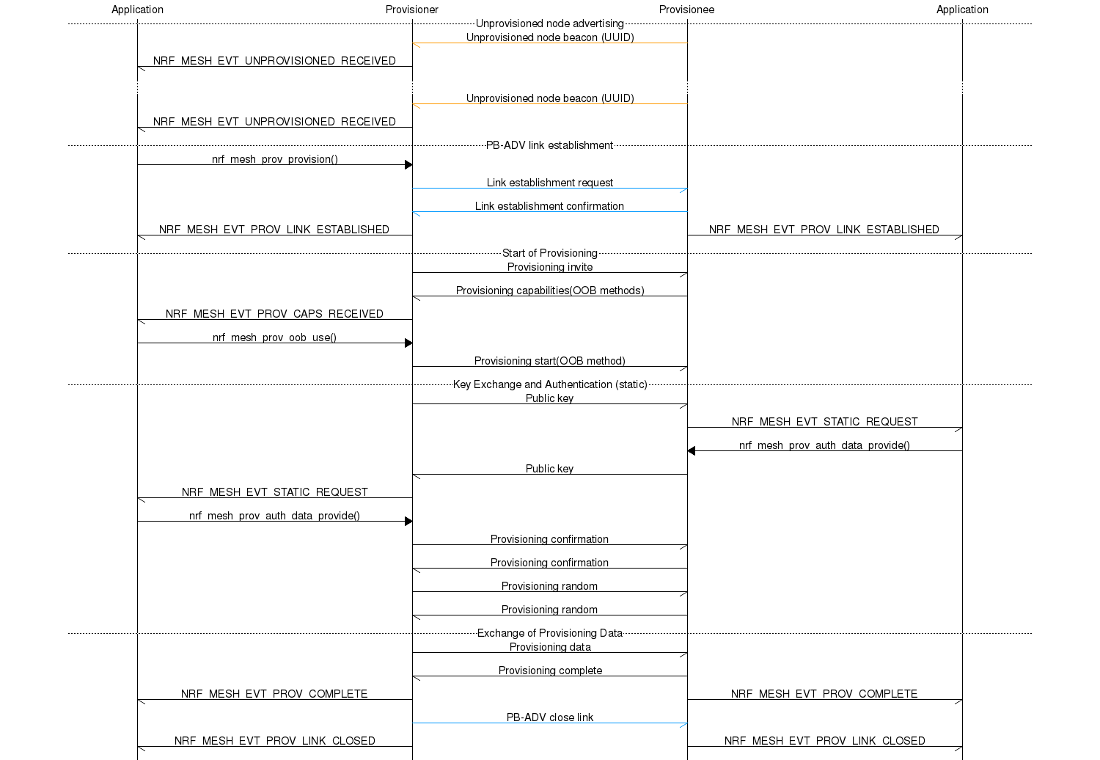
\includegraphics[scale=0.5]{images/provisioning.png}
            		\caption{Provisioning scenarios}
            	\end{center}
            \end{figure}

        \subsection{Thiết bị mới - Provisionee}
        Cách thức hoạt động của một thiết bị mới - unprovisioned hay provisionee: Tiến hành khởi tạo - bao gồm phát beacon để báo rằng mình cần tham gia provisioning, sau đó ở trạng thái chờ sự kiện. Khi bắt được sự kiện yêu cầu kết nối - lời mời provisioning từ provisioner thì đáp lại, tiếp đến chờ đáp lại các sự kiện xác thực, cuối cùng là kết thúc quá trình.
        \begin{figure}[h!]
        	\begin{center}
        		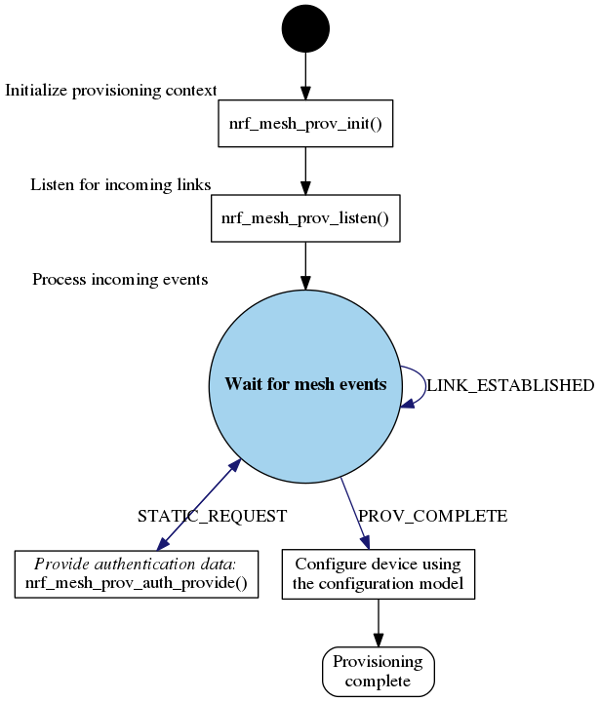
\includegraphics[scale=0.6]{images/provisionee_app_flowchart.png}
        		\caption{Provisionee flowchart}
        	\end{center}
        \end{figure}
	\newpage
        \subsection{Thiết bị Provisioner}
        Là thiết bị hoặc node chịu trách nhiệm thực hiện quá trình provisioning trong mạng mesh. Chúng thường là một phần của các thiết bị gateway - các thiết bị cung cấp một cầu nối giữa mạng mesh và các giao thức kết nối khác.  Cách thức hoạt động của một provisioner: sau các bước khởi tạo thì chờ beacon từ thiết bị mới (unprovisioned), sau đó mời tham gia quá trình provisioning. Trong bước xác thực, tùy theo đối tượng cần provisioning có hay không có hỗ trợ xác thực out-of-band (OOB) mà tiến hành xác thực theo cách tương ứng.
        \begin{figure}[h!]
        	\begin{center}
        		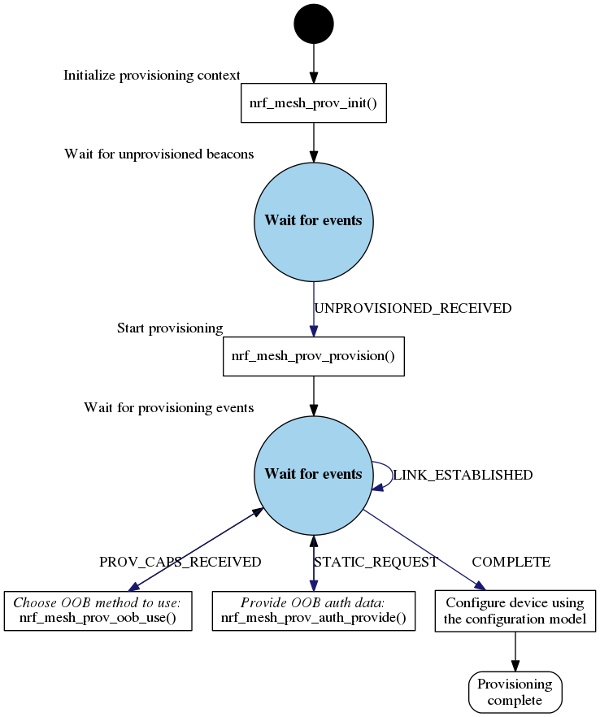
\includegraphics[scale=0.6]{images/provisioner_app_flowchart.png}
        		\caption{Provisioner flowchart}
        	\end{center}
        \end{figure}
        \subsection{Rời khỏi mạng} \label{removenode}
        Sau một thời gian hoạt động, việc phải loại bỏ một số node ra khỏi mạng là điều không thể tránh khỏi, có thể vì nhiều lý do như: node bị hỏng, chuyển node sang một khu vực khác với một mạng mesh khác, thay node mới,... Trong trường hợp nếu không có quy trình loại bỏ node, mạng sẽ đối mặt với nguy cơ bị tấn công kiểu Trashcan, kẻ tấn công có thể khai thác những node bị bỏ đi, lúc này chắc chắn lớp bảo vệ sẽ kém, để lấy thông tin và xâm nhập mạng. Bluetooth Mesh áp dụng 2 bước xử lý sau:
        \begin{itemize}
            \item Cho node bị loại bỏ vào danh sách đen.
            \item Tiến hành cấp lại NetKey cho các node trong mạng trừ node trong danh sách đen. 
        \end{itemize} 

        Quá trình này cần có một thời gian chuyển tiếp, trong thời gian này cả 2 key cũ và mới đều hợp lệ. Sở dĩ cần có thời gian chuyển tiếp này là vì các node low-power thỉnh thoảng mới hoạt động, do đó cần có thời gian để chúng nhận được chìa mới từ node friend của mình.
        \section{Khái niệm Friendship}
       Để có thể ở trong trạng thái sleep lâu dài, các node low power (LPNs) cần tiến hành thiết lập mối quan hệ Friendship với một node ``hàng xóm'' của mình, sau khi thiết lập xong thì node đó trở thành ``friend'' của LPN. Trước khi đi sâu hơn về khái niệm này, chúng ta cần làm quen với một vài tham số:
       \begin{itemize}
	\item ReceiveDelay: Khoảng thời gian từ lúc LPN gửi yêu cầu đến node friend cho đến lúc nó thức dậy lần nữa để bắt đầu nhận dữ liệu. Trong thời gian này LPN vẫn tiếp tục sleep, node friend thì tiến hành chuẩn bị dữ liệu để đáp lại yêu cầu đó.
	\item ReceiveWindow: Khoảng thời gian LPN thức dậy và lắng nghe, lúc này node friend mới có thể gửi dữ liệu cho LPN.
	\newpage
	\begin{figure}[h!]
        	\begin{center}
        		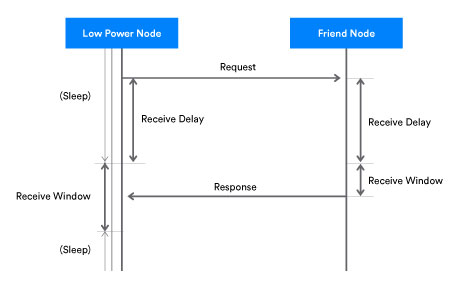
\includegraphics[scale=0.6]{images/friendship-1.jpg}
        		\caption{Hình mô tả ReceiveDelay và ReceiveWindow}
        	\end{center}
        	\end{figure}
        	\item PollTimeout: Khoảng thời gian tối đa giữa 2 lần LPN gửi yêu cầu cho node friend, nếu quá thời gian này mà vẫn không nhận được yêu cầu từ LPN, node friend sẽ kết thúc ``tình bạn'' với nó.
        	\begin{figure}[h!]
        	\begin{center}
        		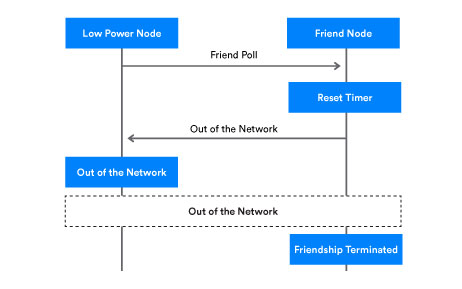
\includegraphics[scale=0.6]{images/friendship-2.jpg}
        		\caption{Hình mô tả PollTimeout}
        	\end{center}
          \end{figure}
       \end{itemize}
       \subsection{Các bước thiết lập Friendship}
       \begin{enumerate}
       \item Node LPN gửi ``yêu cầu kết bạn'', yêu cầu này sẽ không được relay vì nó chỉ có thể kết bạn với những node trong phạm vi kết nối của mình, ngoài ra các node trong phạm vi nhưng không hỗ trợ chức năng Friendship cũng sẽ bỏ qua yêu cầu này. Yêu cầu kết bạn này bao gồm cả 3 thông số ReceiveDelay, ReceiveWindow và PollTimeout.
       \item Node thỏa mãn các yêu cầu để trở thành Friend sẽ gửi lại Friend Offer cho LPN. Gói này bao gồm nhiều tham số như ReceiveWindow có thể hỗ trợ, sức chứa của buffer - buffer này để chứa ``hộ'' các dữ liệu được gửi tới LPN trong lúc nó ngủ và được gọi là Friend Queue,...      
       \item Khi LPN nhận được Friend Offer, nó sẽ dùng một thuật toán để chọn ra 1 Friend (nếu có nhiều Friend Offer), thuật toán này do người phát triển ứng dụng định nghĩa: có thể là ưu tiên node gần hơn hoặc node có khả năng hỗ trợ Friend Queue lớn hơn.
       \item Sau khi đã chọn được Friend, LPN gửi Friend Poll cho node đó.
       \item Sau khi nhận được Friend Poll, node Friend trả lời bằng Friend Update. Mối quan hệ Friendship chính thức được thiết lập.
       \end{enumerate}
       \subsection{Giao tiếp trong Friendship}
       Sau khi đã ``kết bạn'', LPN và node Friend của nó sẽ tiến hành giao tiếp theo các bước sau:
       \begin{figure}[h!]
        	\begin{center}
        		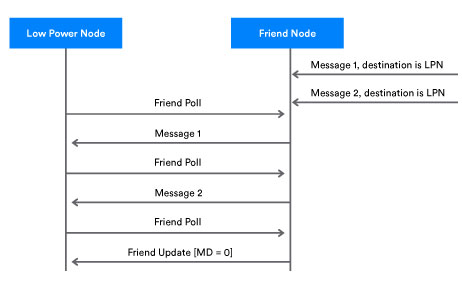
\includegraphics[scale=0.6]{images/friendship-3.jpg}
        		\caption{Hình mô tả quá trình giao tiếp}
        	\end{center}
          \end{figure}
       \begin{enumerate}
	\item Khi node Friend nhận được dữ liệu được gửi đến node LPN là ``bạn'' của nó, nó sẽ lưu vào Friend Queue. Trong hình trên, có thể thấy node Friend đã lưu lại Message 1 và Message 2 thay cho node LPN.
	\item Sau một chu kỳ ngủ, node LPN sẽ gửi yêu cầu Friend Poll đến cho node Friend của mình để kiểm tra có dữ liệu mới hay không.
	\item Nếu có dữ liệu mới, node Friend sẽ gửi ngược lại cho LPN, cứ mỗi lần LPN nhận được dữ liệu nó lại gửi thêm Friend Poll.
	\item Đến khi nào nhận được Friend Update (với tham số More Data = 0) nghĩa là không còn dữ liệu nữa, quá trình giao tiếp này sẽ kết thúc, LPN không gửi Friend Poll nữa.
      \end{enumerate}
      
      Các gói tin giữa node Friend và LPN đều được mã hóa bằng một loại key Friend và chỉ có 2 node này mới có khả năng đọc được.